%----------------------------------------------------------------------------
\chapter{\osszefoglalas} % (Eredmények értékelése)
%----------------------------------------------------------------------------

%----------------------------------------------------------------------------
\section{Eredmények}
%----------------------------------------------------------------------------

Ennek a dolgozatnak a célja egy mérő- és visszajelzőrendszer fejlesztése, amely egy mezőgazdasági gép adapteréhez szolgáltat biztonságtechnikai jelzéseket. A jelzések egy tárcsás nyomatékhatároló működéséről adnak biztosítékot, amely meggátolja, hogy egy bizonyos mértékű nyomaték az adapteren működő tengelyeket terhelje. Ezen felül a rendszer a monitorozott három tengely fordulatszámáról is ad számszerű visszajelzést. A nyomatékhatároló előtti és utáni tengely-fordulatszám összehasonlításával lehet az eszköz megcsúszását jelezni, amelyhez két szenzort alkalmaztam, valamint egy harmadikat amely a takarmány felszedését végző tengely fordulatszámát méri.

A feladat nagy része a környezethez és alkalmazáshoz megfelelő eszközök választása volt. A gépek hajtásánál, ahol a tengelyek mérése történik, a zsír és por az általános, így olyan szenzorra volt szükség, amely ezek mellett is pontosan működik. Az érzékelést három induktív ipari szenzor végzi, amelyek kialakításuktól fogva védve vannak a szennyeződésektől, és az elektromágneses terek változásait érzékelik, így a mérést sem befolyásolják a szennyeződések sem a levegőben, sem a felületen lerakódva. Ahol lehetett, lánckerekek fogainak mérését végeztem, ezáltal nem kellett sok támogató tervezés, ahol pedig nem állt rendelkezésre ez a módszer, ott egy fogas hajlított lemez mérése valósul meg. A rendszer irányítását egy programozható relé végzi, amely egy PLC ipari vezérlőegység egyszerűbb és kisebb változata. Ezt többek között az adapteren található $12$~V tápfeszültség határozta meg, amit a rendszer többi részének megtervezésében is figyelembe vettem. A berendezés egy úgynevezett Létra Diagrammos programozási felülettel rendelkezik, amellyel a kapott analóg jeleket feldolgozni, így fordulatszámmá konvertálni lehet. Ezek után a rendszer elvégzi az összehasonlítást, és a fordulatszámokat egy felhőbe felküldi, valamint szükség esetén az adapteren található ipari lámpát is felkapcsolja. Az ipari lámpa az egész rendszer házaként szolgáló szennyeződésmentes doboznak az oldalán található, és abban az esetben villog, ha a nyomatékhatároló megcsúszott.

A dolgozat produktuma ez a rendszer, amelynek tervezése során sokat tanultam az önálló fejlesztési munka kihívásairól, a "megrendelő" céggel való kapcsolatépítésről. A projekt összetettsége miatt, számos különböző forrástól kértem segítséget, támogatás, ami nagyban hozzájárult a munkám sikerességéhez.

%----------------------------------------------------------------------------
\section{Továbbfejlesztési lehetőségek}
%----------------------------------------------------------------------------

\subsection{Alternatív kialakítású nyomatékhatároló}

A Hevesgép Kft. által gyártott felszedő adaptereken egy alternatív, silózó felé elhelyezett nyomatékhatároló is létezik, amely a \ref{hatso_nyomhat} képen látszik. A feladat továbbfejlesztéseként ennek a nyomatékhatárolónak a ki- és bemeneti oldalának a fordulatszámmérése is megvalósítható. A nehézségét fokozza, hogy ez a tengely az adapter külsején helyezkedik el, valamint a fordulatszáma is jóval magasabb, mint a dolgozatban számolt elrendezésnek, hiszen ez a silózóból érkező közvetlen fordulatszámot továbbítja ($340 - 680$~rpm).
\begin{figure}
	\centering
	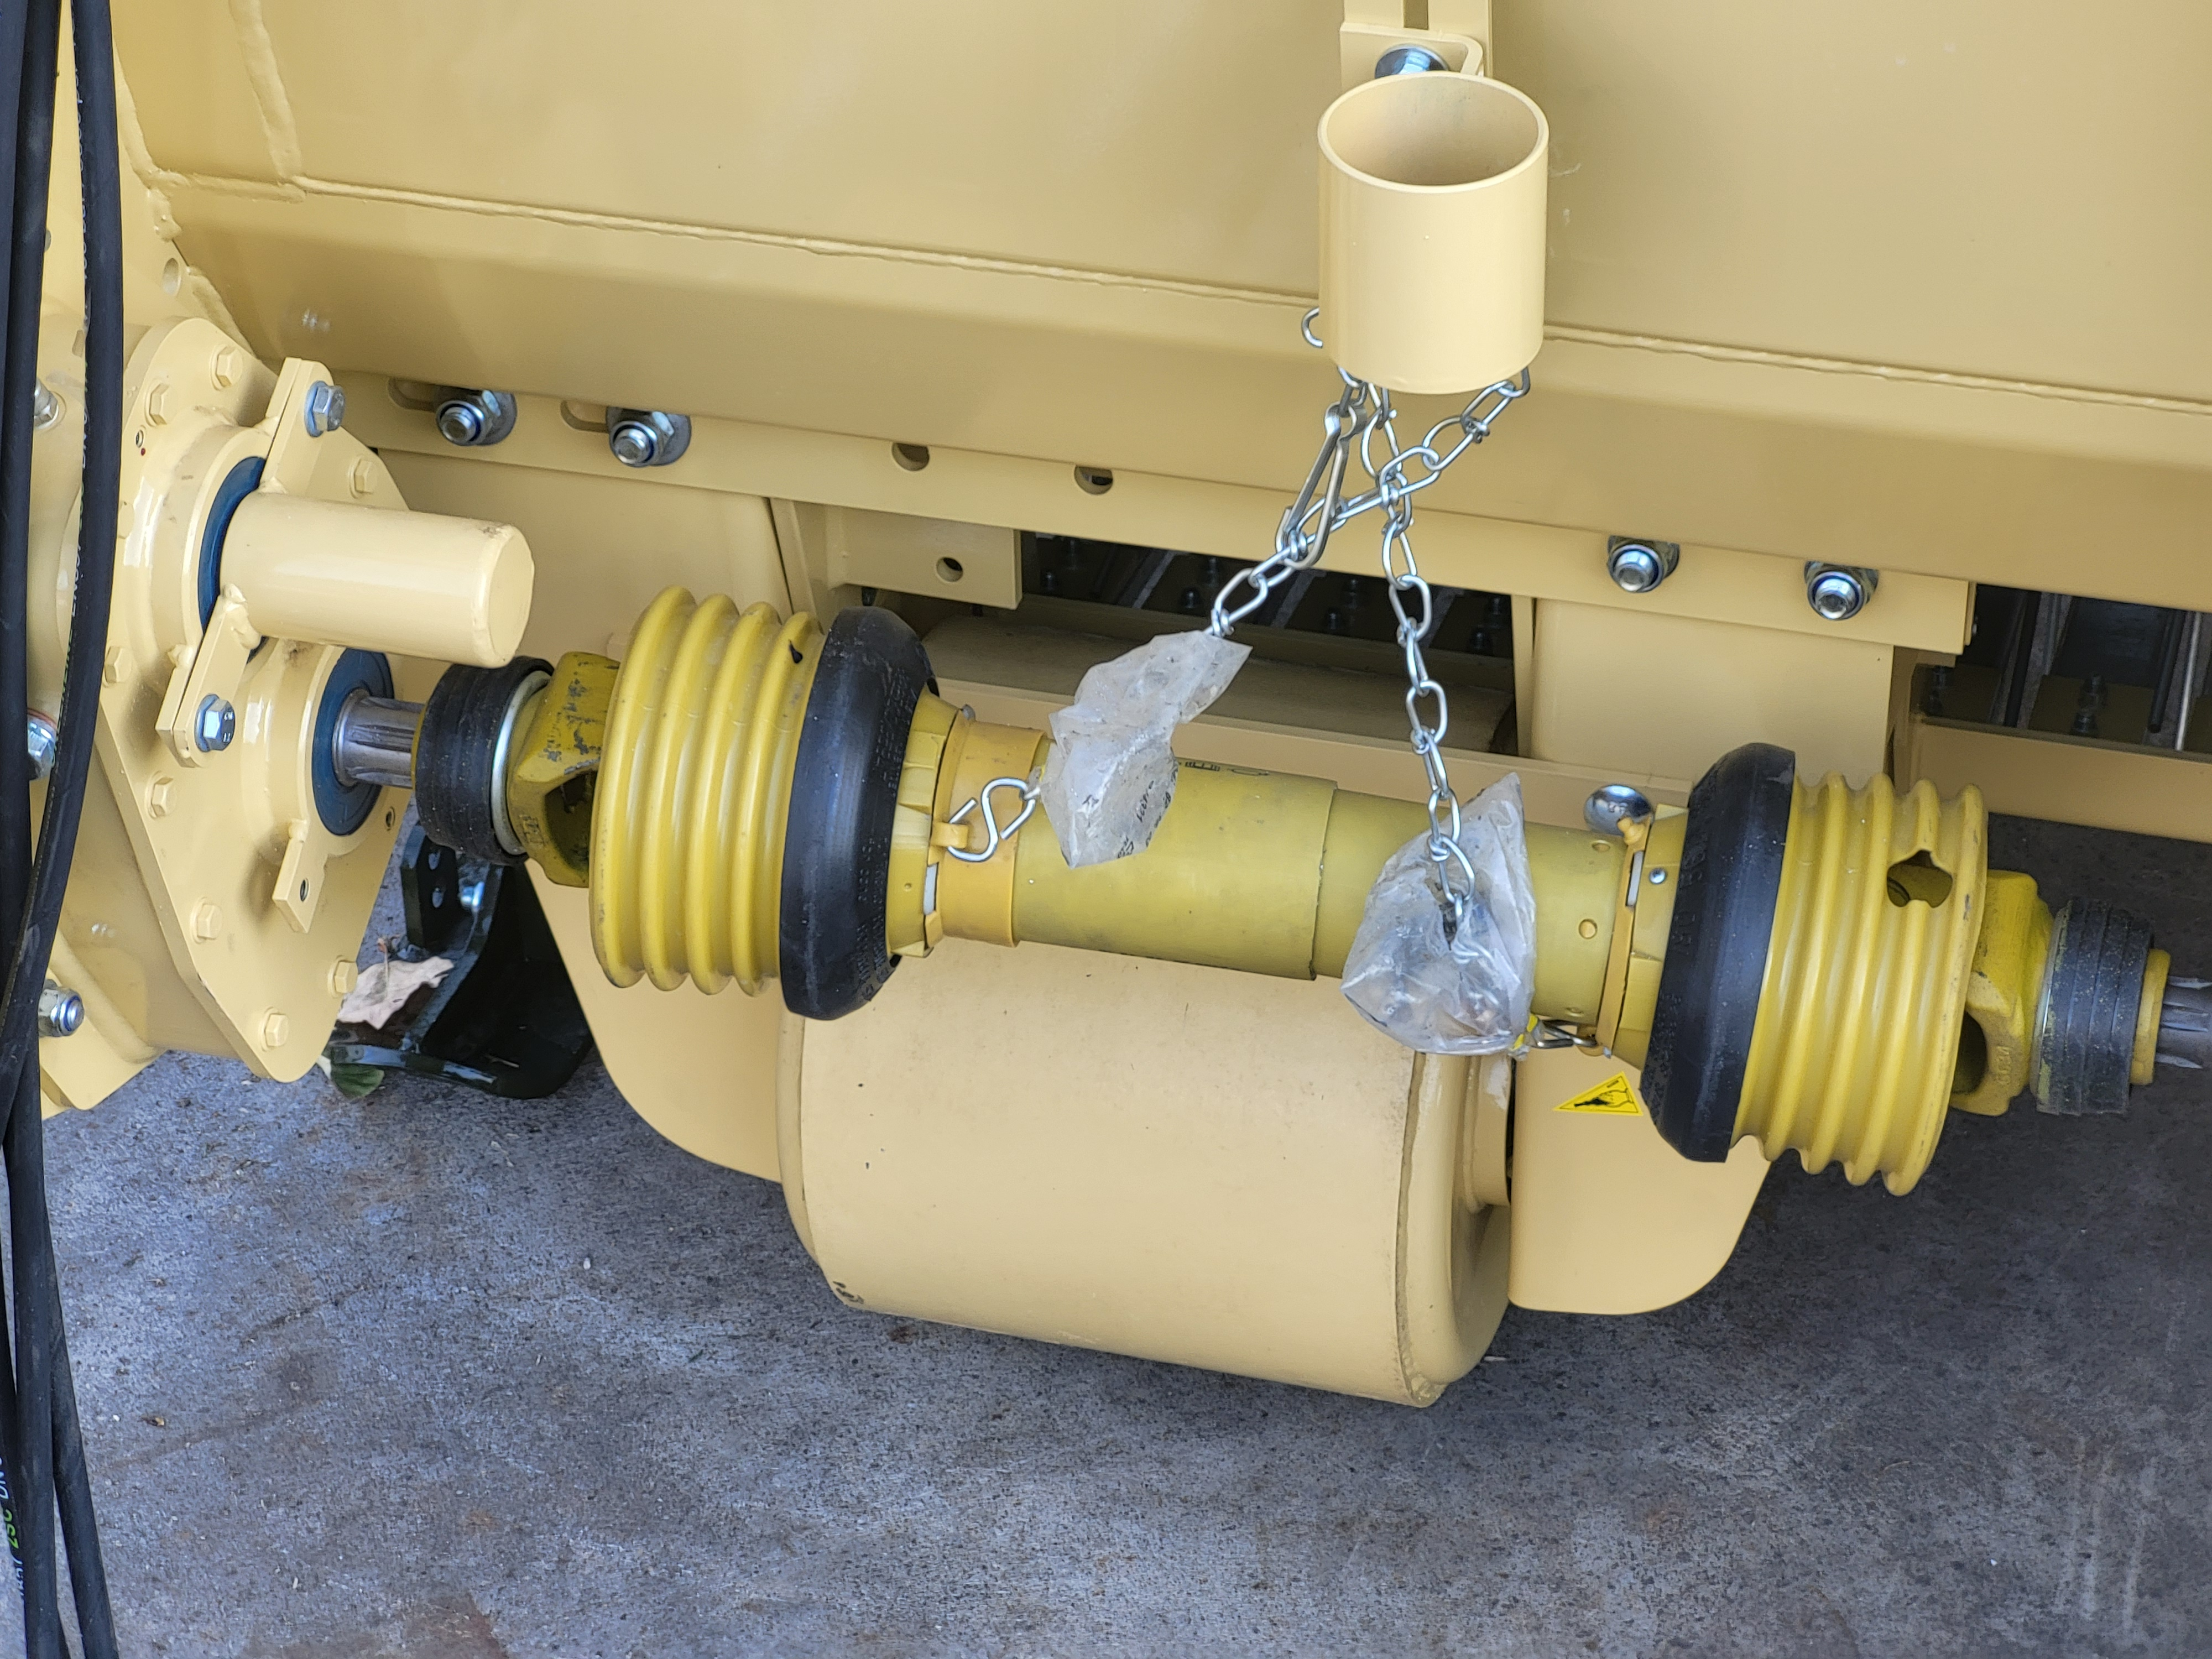
\includegraphics[width=\columnwidth*7/10]{figures/hatso_nyomatekhatarolo.jpg}
	\caption{Az alternatív, hátsó oldali nyomatékhatároló képe.}
	\label{hatso_nyomhat}
\end{figure}

\subsection{Gyártói szabványos kommunikáció}

Ahogyan a \ref{visszajelz} fejezetben említésre került, az adapter silózóval való csatlakozásánál, többek között, jelek átadására is van lehetőség. Az egyes gyártók eltérő kialakítású csatlakozókat használnak, így a berendezésnek nagy előrelépés lenne, ha minden egyes szabványos csatlakozó fel lenne térképezve -- ehhez a gyártókkal kéne egyeztetni --, hiszen sok lehetőséget megnyitna a fejlesztés szempontjából. Ezen az úton a silózó fülkéjében található kijelzők és tájékoztató berendezésekhez hozzáférést kapna a rendszer, így integrálva lehetne bizonyos információkat átadni, amelyhez természetesen az összes visszajelzőrendszer ismerete is szükséges lenne.

\subsection{Kivitelezés}

Talán a feladat legkézenfekvőbb továbbfejlesztési lehetősége, a berendezés alkatrészeinek megrendelése, felszerelése, a szoftver felprogramozása és a rendszer kipróbálása, letesztelése, megvalósítása.

% Keltezés, aláírás
\vspace{0.5cm}

\begin{flushleft}
{Budapest, \today}
\end{flushleft}

\begin{flushright}
\emph{\authorName}
\end{flushright}

\vfill
